\section{Schlüsse aus der Analyse}

Die in der Analyse festgestellten Ansätze und Anforderungen legen eine Grundlage für ein Systemkonzept vor, welches nun in diesem Kapitel beschrieben wird, während eine Teil-Implementierung im folgenden Kapitel 4 erfolgt.

Für ein den Anforderungen entsprechend skalier- und erweiterbares System muss dieses nicht nur modular, sondern auch dezentral ausführbar konzipiert werden. Gerade die Skalierbarkeit von Multi-User Zugängen und angesteuerten Geräten und Robotern ist dabei von zentraler Bedeutung. Dadurch sind einige der betrachteten Roboter-Lösungen, wie die in der Arbeit von Inoue et al. \cite{meanField} beschriebene, von vornherein nicht anwendbar, da sie eine zentrale Steuerung voraussetzen. Damit das Gesamtsystem möglichst robust ist, sollte neben der Steuerung auch die Planung möglichst verteilt stattfinden, sodass einzelne Fehler oder fehlerhafte Befehle nicht die Gesamtplanung beeinträchtigen.

Zu diesem Zweck ist eine Anwendung von den Ansätzen von Yang et al. \cite{2DPlan} und Reily et al. \cite{silentSwarm} nützlich. Indem die Position von einzelnen Gegenständen zentral verwaltet wird, kann die detaillierte Navigation zu diesen Gegenständen an die einzelnen Roboter ausgelagert werden. Die dadurch erstellten Zielpunkte können gleichzeitig auch mit anderen Robotern geteilt werden, sodass Roboter nach der von Reily et al. \cite{silentSwarm} vorgestellten Methode Kollisionen vermeiden können. Dadurch muss das zentrale System nur die genannten Positionen der zu transportierenden Gegenstände und die Zielkoordinaten bereitstellen können, um eine möglichst kollisionsfreie Navigation der Roboter zu ermöglichen.

Um einen sicheren Nutzerzugang mit zugänglicher Semantik zu ermöglichen, muss zwingend ein nutzerzentriertes UX Konzept entwickelt werden, bevor ein solches System zum Einsatz gebracht werden kann. Ein solches Konzept entspricht jedoch nicht dem Rahmen des Forschungsprojekts, weshalb das hier vorgestellte Konzept von einer späteren Umsetzung einer universellen Schnittstelle ausgeht. Um eine solche Nutzerschnittstelle zu ermöglichen, müssen die benötigten Interaktionen im Vornherein festgelegt werden. Diese werden im Unterkapitel des User Interface-Knotens dargelegt.


\FloatBarrier
\newpage \section{Systemarchitektur}

\begin{figure}[h]
\centering
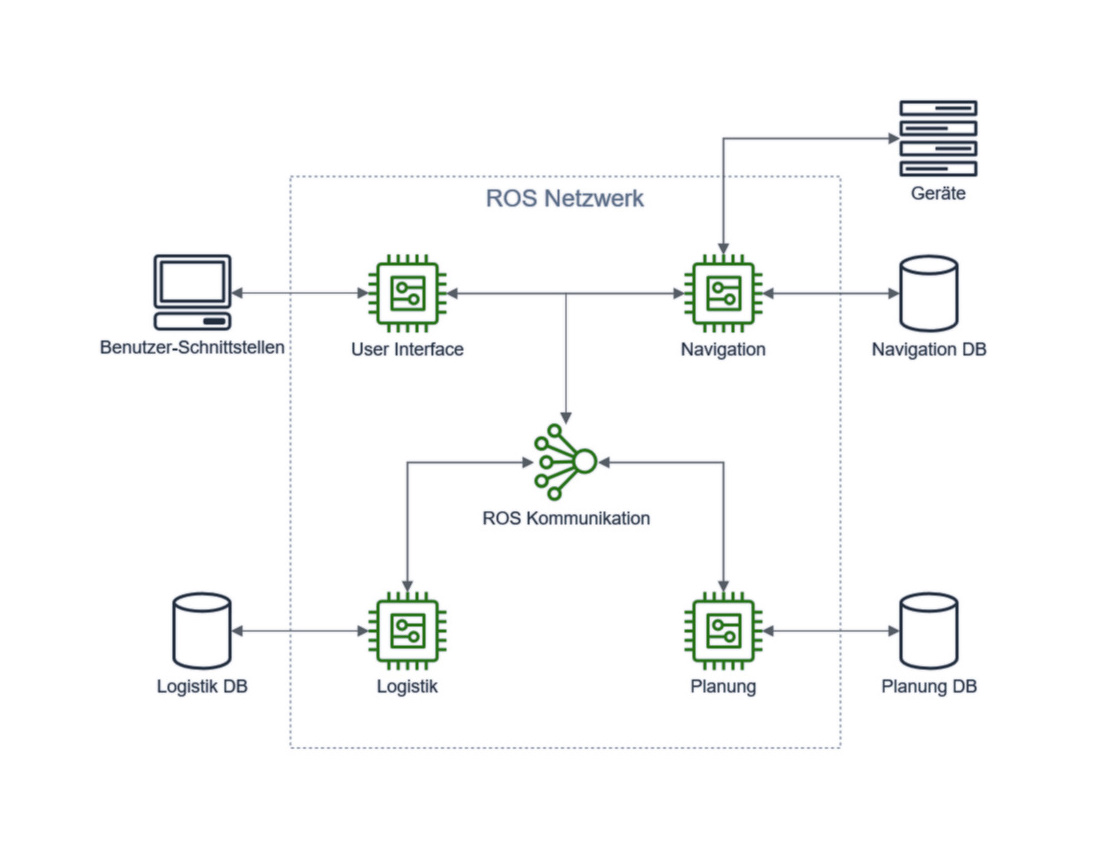
\includegraphics[width=\textwidth]{Bilder/3_ROS_Netzwerk.jpg}
\caption{Systemarchitektur}
\end{figure}

Das System ist im Kern um vier Knoten herum aufgebaut: User Interface, Logistik, Planung und Navigation. Diese vier Knoten kommunizieren untereinander, um die verschiedenen Aufgaben des Systems gemeinsam lösen zu können. Dazu umfassen der Planungs-, Navigations- und der Logistik-Knoten jeweils Datenbanken, um Pläne und Szenarien beziehungsweise Geräte und Navigationskarten sowie die verschiedenen Vorräte im Lager zu verwalten. Der Navigationsknoten unterstützt dazu die Steuerung der einzelnen Geräte, während der User Interface-Knoten die Kommunikation mit Nutzern ausführt.

Die Kommunikation zwischen den Knoten wird in den Beschreibungen der einzelnen Knoten näher erläutert. Vor allem sollte hier eine Kommunikationsart verwendet werden, die es ermöglicht, Anfragen und Befehle zwischen Knoten im System zu senden. Die Arten von Befehlen, die zur Ausführung nötig sind, werden in den Beschreibungen der einzelnen Knoten in Tabellen exemplarisch dargestellt. Dabei werden sowohl die Nachricht als auch die erwarteten Antwortmöglichkeiten als symbolischer Satz erläutert, ohne sich auf ein bestimmtes Nachrichtenformat festzulegen.

Die Kommunikation mit den Nutzern soll unabhängig über die verwendete Plattform stattfinden. Dies wird über eine generische Schnittstelle im User Interface-Knoten realisiert, die über eine Netzwerkverbindung auch ermöglicht, von externen Geräten auf das System zuzugreifen. So ist für die nachträgliche Erweiterung um neue Nutzerschnittstellen keine Änderung am System selbst nötig. Für den Entwurf dieser Benutzeroberflächen ist eine eigene UX-Konzeptionierung nötig, um die Anforderungen an eine zugängliche Semantik zu erfüllen. Da davon ausgegangen werden kann, dass die Form der Benutzeroberfläche keinen Einfluss auf die innere Funktionsweise des Systems hat, wird diese jedoch hier als gegeben angenommen.

Die Kommunikation mit den verbundenen Geräten muss ebenfalls über eine Netzwerkverbindung realisiert werden, da gerade mobile Roboter zwangsläufig nicht Teil derselben Maschine sein können. Es wird jedoch davon ausgegangen, dass sie als Teil desselben internen Netzwerks angenommen werden können, um die Kommunikation zu erleichtern und die Verbindungssicherheit zu gewährleisten. Auch wird die Steuerungsprogrammierung der eigenen Roboter als gegeben angenommen, da der Systementwurf darauf ausgelegt wird, dass die explizite Steuerung nicht durch das System durchgeführt wird. Der Entwurf der Navigationsalgorithmen ist eine eigene Forschungsaufgabe für sich, sodass hier nicht versucht wird, diese nebensächlich zu lösen.

Eine zentrale Herausforderung beim Transport von Möbeln ist, dass der Roboter in der Lage sein muss, den gewünschten Gegenstand zu identifizieren. Da größere Möbel wie Krankenliegen nicht in einem standardisierten Regal aufbewahrt werden können, muss auf eine Form der Objekterkennung zurückgegriffen werden. Es wird dafür vorausgesetzt, dass die Roboter so konzipiert sind, dass sie in der Lage sind, einen bestimmten Gegenstand zu identifizieren, wenn sie sich in der unmittelbaren Nähe befinden. Dann kann eine angepasste Version des von De La Puente et al. in \cite{assistRobot} vorgestellten Algorithmus verwendet werden, um den Gegenstand aufzuheben. Für das hier vorgestellte System wäre es dabei unerheblich, ob die Ausführung des Objekterkennungsalgorithmus auf den Robotern selbst oder einem externen Server durchgeführt wird.

Die Ausführung der Aufgabe kann dann über die von Yang et al. \cite{2DPlan} vorgestellte Methode erfolgen. Dabei wird ein Pfad von der derzeitigen Roboter-Position zu der Endposition der Aufgabe über die derzeitige Position des zu transportierenden Gegenstands geplant. Dies kann in der Regel auf einzelnen Robotern ausgeführt werden, sodass das System diese Rechenleistung nicht zur Verfügung stellen muss. Dies hat den Vorteil, dass es auf den jeweiligen Robotern vorgenommen werden kann und nur eine geringe Kommunikation mit dem zentralen Server benötigt.

Es wird sich bei der Navigation der Roboter in Situationen, in denen sie als Schwarm agieren müssen, an den Arbeiten von Reily et al. \cite{silentSwarm} orientiert. Da alle Roboter in demselben Netzwerk liegen, können sie sich gegenseitig erkennen und miteinander kommunizieren. Durch das Abrufen von Zielpunkten und Navigationskarten vom Navigationsknoten können einzelne Roboter die Wege anderer Roboter voraussagen und sich so gegenseitig ausweichen. Die Voraussetzung, dass jeder Roboter in der Lage ist, mehrere Wegplanungen gleichzeitig auszuführen, muss dafür als gegeben angenommen werden. Die Rechenlast der Wegplanung auf den einzelnen Robotern kann dadurch verringert werden, dass die Roboter auf die im Navigationsknoten liegende Karte zurückgreifen können, anstatt selbst eine erstellen zu müssen.



\FloatBarrier
\subsection{Datenbanken}

Die Datenbank des Logistik-Knotens verwaltet alle Vorräte, die vom System verwendet werden. Für das System sollte es dabei unerheblich sein, welchen individuellen Gegenstand eines Vorrats es verwendet, weshalb dieses für jeden Gegenstand eine Art festhält, nach der gesucht werden kann. Über diese Gegendstandsart kann auch, wenn erforderlich, eine genaue Spezifizierung bei zum Beispiel gesonderten Nutzungsrechten erfolgen.

Da es für den Transport durch Roboterplattformen nicht ausreicht, nur die Existenz von Gegenständen festzuhalten, muss neben der Art auch die Position im Skills Lab oder Lager festgehalten werden. Dabei sollte es auch ermöglicht werden, dass eine Art von Gegenständen über mehrere Positionen verteilt gelagert werden kann. Daher verfügt jeder individuelle Gegenstand, auch wenn dieser ansonsten identisch mit anderen in der Datenbank ist, über eine eigene Position, welche als Koordinatenpunkt festgehalten wird. Diese sind der Karte, welche dem Navigationsknoten vorliegt, zugeordnet.

Dazu ist es für die zeitkritische Planung wichtig, dass die Verfügbarkeit nicht nur zum jeweiligen Zeitpunkt festgehalten wird, sondern auch für mehrere Zeitpunkte in der Zukunft. Dementsprechend kann die Verfügbarkeit nicht nur ein Attribut eines Gegenstands sein, sondern muss auch selbstständig festgehalten werden. Deshalb muss die Datenbank in zwei verschiedene Tabellen, eine für die Suche nach Gegenständen und eine für die Suche nach Verfügbarkeiten, unterteilt werden. Dadurch kann der Logistik-Knoten ohne komplexe Algorithmen oder doppelte Einträge von Gegenständen Anfragen beantworten.

Die Datenbank des Planungsknotens ist ähnlich aufgebaut, wird aber in drei getrennten Tabellen implementiert. Die erste Tabelle fasst Szenarien mit einer für Menschen verständlichen Beschreibung sowie einen Satz für Geräte verständlicher Anweisungen. Dadurch kann sie genutzt werden, um Nutzern vorgefertigte Szenarien zur Auswahl anzubieten sowie als Grundlage der Robotersteuerung zu dienen. Dazu muss auch die Art von Gegenständen, die für jedes Szenario benötigt wird, sowie die Art des Raums, in denen dieses Szenario durchgeführt werden kann, festgehalten werden. Szenarien werden jedoch nicht für sich selbst ausgeführt, sondern fassen in erster Linie nur Befehle in einem Datenpaket zusammen, um die Planung zu erleichtern.

Um diese umzusetzen, werden geplante Szenarien in einer zweiten Tabelle eingetragen, welche die konkreten Pläne mit den dafür benötigten Geräten, spezifischen Gegenständen sowie den dafür vorgesehenen Raum umfasst. In dieser wird Szenarien zudem eine Zeitspanne zugeordnet, zu welchen diese umgesetzt werden. Sie fungiert so auch als Warteschlange, welche der Planungsknoten zu den jeweiligen Zeitpunkten in Befehle für die Navigation umwandeln kann.

Da davon ausgegangen werden kann, dass es in einem Skills Lab mehrere identisch aufgebaute Simulationsräume geben kann, werden die verfügbaren Räume in einer dritten Tabelle gespeichert, welche neben der Raumnummer auch die Art des Raums, wie sie in den Szenarien eingetragen ist, umfasst. Dadurch kann ein Plan spezifizieren, in welchem Raum er umgesetzt wird, auch wenn das Szenario auf andere, identisch aufgebaute Räume angewendet werden kann.

Die Datenbank des Navigationsknotens speichert die angeschlossenen Geräte, deren Verfügbarkeit sowie Einsatzmöglichkeiten. Der genaue Status der Geräte wird hier nicht gespeichert, da er flüchtig ist und sich insbesondere bei mobilen Robotern kontinuierlich ändern kann. Daher ist diese Datenbank ähnlich der Datenbank des Logistik-Knotens aufgebaut, die Verfügbarkeit wird genauso über eine zweite Tabelle in der Datenbank festgehalten. Statt einer Gegenstandsart wird hier jedoch über eine Liste von Schlüsselwörtern festgehalten, welche Funktion ein Gerät erfüllen kann. Dies ist vor allem für Roboter vonnöten, welche nur bestimmte Gegenstände transportieren können.



\FloatBarrier
\subsection{User Interface}

\begin{figure}[h]
\centering
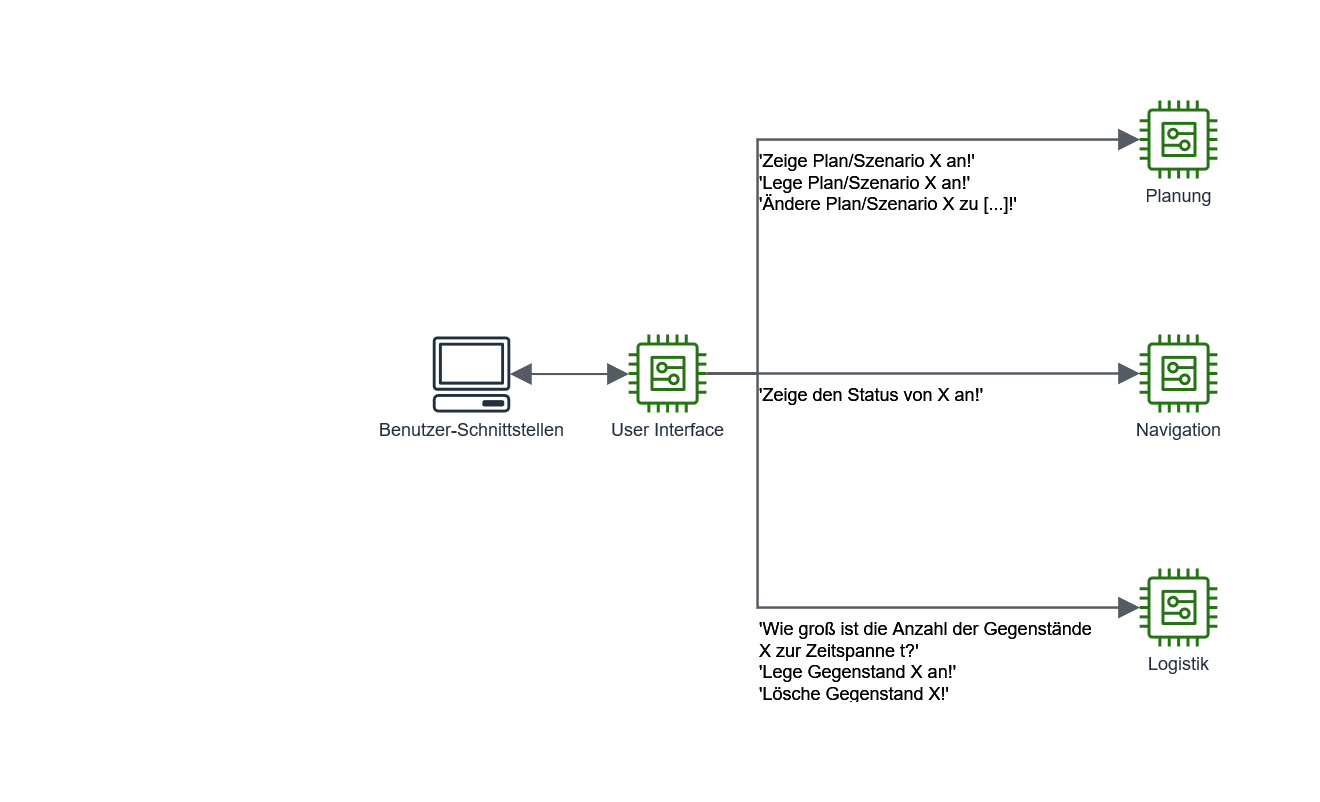
\includegraphics[width=\textwidth]{Bilder/3_User_Interface.png}
\caption{User Interface-Knoten}
\end{figure}

Der User Interface-Knoten stellt den Teil des Systems dar, mit dem Nutzer interagieren können. Er verwaltet die Kommunikation zu Nutzerschnittstellen, kann auf Anfrage Daten der Logistik, Planung und Navigation anzeigen und bündelt den Informationsfluss nach außen. Der Knoten ist auch für die Anzeige und Protokollierung von Fehlermeldungen verantwortlich. Für die Aufnahme dieser ist er in der Lage, einen gemeinsamen Kanal abzurufen und Nachrichten an diesen anzuzeigen.

Die Eingabe von auszuführenden Anweisungen an das System soll nur über den Planungsknoten erfolgen, um zu verhindern, dass Nutzerbefehle die Ausführung laufender Pläne und Szenarien stören, und zu ermöglichen, dass das System vorher überprüfen kann, ob Kollisionen mit diesen vorliegen. Daher übersetzt der User Interface-Knoten diese Nutzerbefehle nur in Systemanweisungen und leitet sie an den Planungsknoten weiter.

Hierfür werden zwei verschiedene Arten von Anweisungen verwendet. Die erste soll dazu genutzt werden, ein neues Szenario zu erstellen oder ein bestehendes anzupassen. Diese können gut zusammengefasst werden, da Szenarien nur der Vorbereitung von Handlungen dienen, aber keine Reservierungen von Geräten und Gegenständen benötigen. Die zweite Art von Anweisung soll einen neuen Plan anlegen oder einen bestehenden verändern. Damit soll es auch möglich sein, aktuell laufende Aktionen der Roboter abzubrechen oder Pläne zu löschen, da dies gut als 'einen Plan ändern' umgesetzt werden kann. Diese beiden Anweisungen werden getrennt betrachtet, da letztere eine Prüfung der verfügbaren Ressourcen und einen deutlich höheren Aufwand des Systems erfordern. In beiden Fällen soll der Nutzer aber eine Rückmeldung vom System über die vorgenommene Handlung erhalten.

Es kann unter Umständen nötig sein, dem System mitzuteilen, dass einzelne Gegenstände manuell hinzugefügt oder entfernt wurden. Dabei kann nach demselben Schema wie bei der Bearbeitung von Szenarien vorgegangen werden, da entweder eine neue Art von Gegenstand der Logistik hinzugefügt wird oder der Eintrag eines bestimmten Gegenstands verändert wird.

Um einzelne Geräte, Gegenstände, Pläne oder Szenarien anzuzeigen, kann zwischen dem User Interface-Knoten und den entsprechenden Knoten eine direkte Kommunikation stattfinden. Da hier davon ausgegangen wird, dass Nutzer keine kontinuierlichen Daten anfragen werden, kann auch hier eine Anweisung verwendet werden, die die verbundenen Knoten zu einer Anfrage auf die Datenbank veranlasst und die angeforderten Daten als Antwort zurückgibt.



\FloatBarrier
\newpage \subsection{Planung}

\begin{figure}[h]
\centering
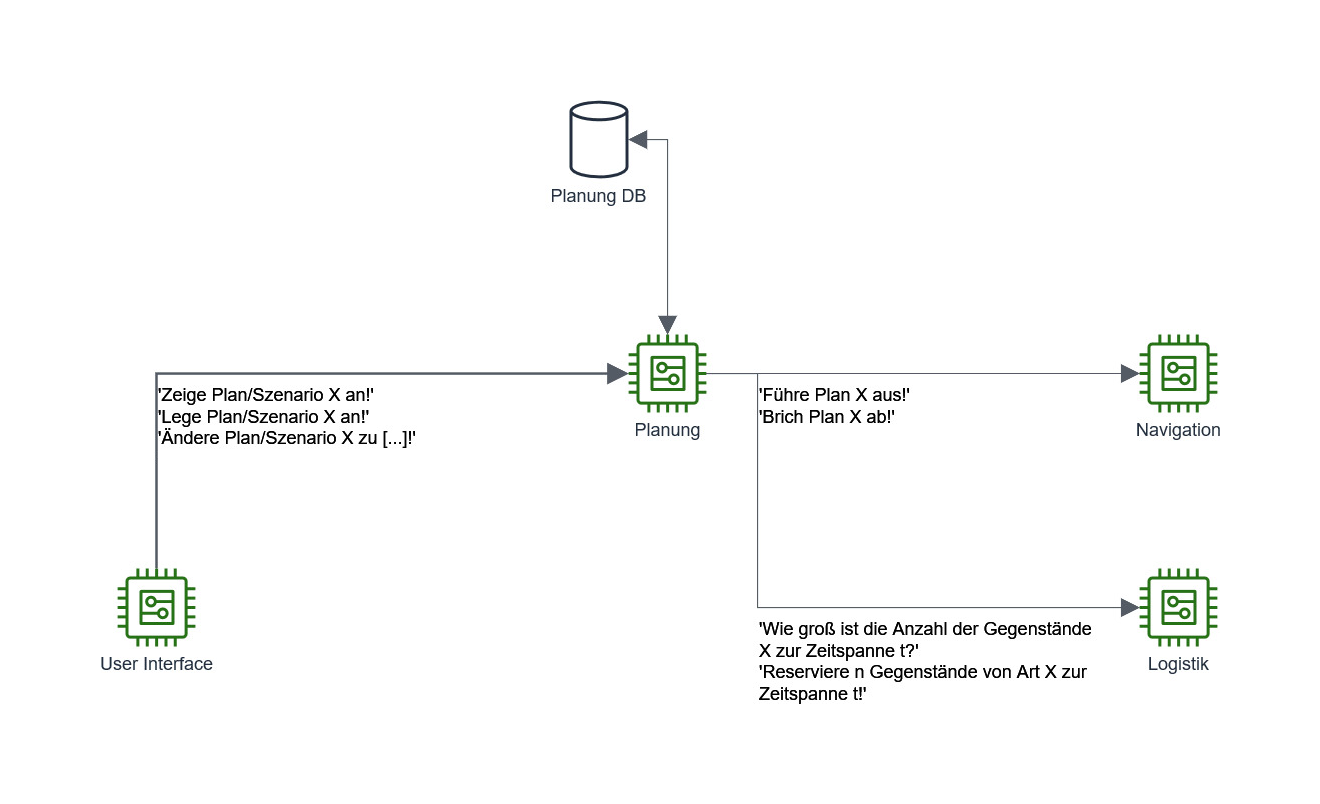
\includegraphics[width=\textwidth]{Bilder/3_Planung.png}
\caption{Planungsknoten}
\end{figure}

Die Hauptaufgaben dieses Knotens sind, Systemanweisungen von Nutzern in einzelne Befehle umzuwandeln und die erstellten Szenarien zu verwalten. Dazu muss es sowohl mit dem Logistik- als auch dem Navigationsknoten und den dazugehörigen Datenbanken kommunizieren können. Die Datenbank des Planungsknotens beinhaltet die Details der angelegten Szenarien und die zu einer bestimmten Zeit auszuführenden Pläne, wie oben beschrieben. Da davon ausgegangen wird, dass sich die Räume eines Skills Labs nicht ändern, müssen Nutzer nur direkt auf Pläne und Szenarien zugreifen können. Für das Anlegen oder Ändern von Plänen müssen zunächst die konkreten Verfügbarkeiten von Gegenständen und Geräten erfragt werden, was der Planungsknoten automatisch für den Nutzer ausführt. Basierend auf den Verfügbarkeiten gibt er dem Nutzer Feedback, ob ein Plan umsetzbar ist und trägt diesen gegebenenfalls auch in die Warteschlange der Pläne ein.

Damit Pläne umgesetzt werden, muss der Knoten selbstständig überprüfen, welcher als nächstes auszuführen ist, um zu dem angegebenen Zeitpunkt die entsprechenden Anweisungen an den Navigationsknoten geben zu können. Der Planungsknoten stellt dadurch das zentrale Element bei der Ausführung von vorher festgelegten Szenarien dar. Der Navigationsknoten gibt den Status der momentan ausgeführten Pläne dabei an den Planungsknoten zurück. Dadurch kann der Planungsknoten die an die Navigation gegebenen Anweisungen überwachen und gegebenenfalls die Planung anpassen. Falls ein Plan während der Ausführung geändert wird, wird der Navigationsknoten informiert, dass die jeweilige Aktion abgebrochen wird. Danach sendet der Planungsknoten einen neuen Plan, um die Änderungen umzusetzen. Auch hier wird eine Rückmeldung des Navigationsknotens erwartet, bis eine Bestätigung erfolgt, dass die Aktion vollständig abgebrochen wurde.

Ein Nutzer kann über das User Interface auf den Planungsknoten zugreifen, um neue Pläne und Szenarien anzulegen, bestehende anzuzeigen oder zu ändern. Der Knoten prüft bei neu angelegten oder geänderten Einträgen, ob dieser ausgeführt werden kann, indem entsprechende Anweisungen an die Logistik- und Planungsknoten gesandt werden. Falls dies der Fall ist, übersetzt der Knoten die ursprüngliche Anweisung in eine Datenbankanfrage und gibt zuletzt das Ergebnis als Rückmeldung zurück.

\begin{table}[h]
\begin{center}
\begin{tabular}{| r l |}
  \hline
  Anweisung  & \dq Zeige Plan/Szenario X an!\dq  \\
  \hline
  Rückmeldung & \dq Plan/Szenario X umfasst [..].\dq  \\
  oder     & \textbf{\dq Plan/Szenario X ist nicht bekannt.\dq } \\
  \hline
  \hline
  Anweisung  & \dq Lege Plan/Szenario X an!\dq  \\
  \hline
  Rückmeldung & \dq Plan/Szenario X angelegt.\dq  \\
  oder     & \textbf{\dq Plan/Szenario X existiert schon.\dq } \\
  \hline
  \hline
  Anweisung  & \dq Ändere Plan/Szenario X zu [..]!\dq \\ 
  \hline
  Rückmeldung & \dq Plan/Szenario X umfasst [..].\dq  \\  
  oder     & \dq Vorrat für Plan/Szenario X nicht ausreichend.\dq \\
  oder     & \textbf{\dq Plan/Szenario X ist nicht bekannt.\dq }\\
  \hline
  \hline
\end{tabular}  
\caption{Kommunikation von User Interface zu Planung}
\end{center}
\end{table}


\FloatBarrier
\newpage \subsection{Navigation}

\begin{figure}[h]
\centering
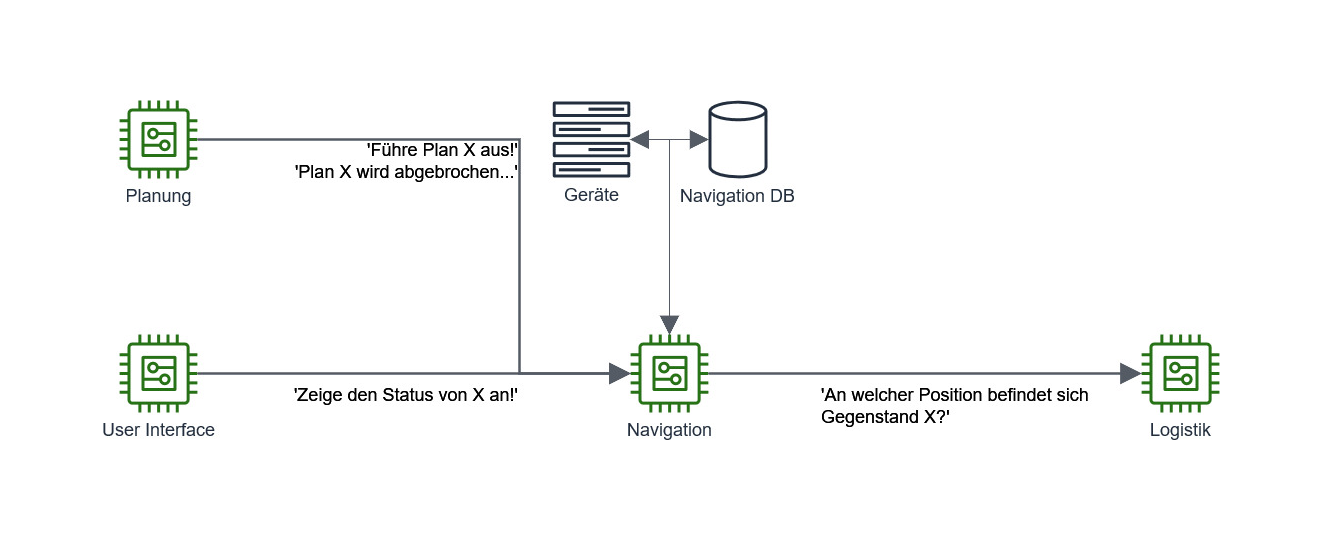
\includegraphics[width=\textwidth]{Bilder/3_Navigation.png}
\caption{Navigationsknoten}
\end{figure}

Der Navigationsknoten ist für die Steuerung der verbundenen Geräte, insbesondere der Roboter, nach den übermittelten Anweisungen des Planungsknotens verantwortlich. Er wandelt diese in für die Roboter ausführbare Navigationsanweisungen um und überwacht den Status der Geräte während der Ausführung.

Der Planungsknoten wird im laufenden Betrieb den Großteil seiner Anfragen an die Navigation senden. Dies erfolgt über zwei Arten von Anweisungen. Die erste weist die Navigation an, einen Plan auszuführen, der in der Nachricht spezifiziert wird. Ein solcher Plan beinhaltet ein Szenario, den Raum, in dem dieses umgesetzt werden soll, sowie die Gegenstände, die verwendet werden sollen. Aus diesen berechnet der Navigationsknoten die Route von geeigneten Geräten und gibt diesen die entsprechenden Befehle.

Um dies umzusetzen, muss der Knoten über eine Navigationskarte verfügen, die das gesamte Skills Lab inklusive Lager umfasst. Dazu muss eine Datenbank der ansprechbaren Geräte entsprechend der oben beschriebenen Vorlage angebunden sein. Aus dieser Datenbank kann der Planungsknoten die zu verwendenden Geräte für eine Handlung auswählen, um ihnen dann die Anweisungen zu erteilen. Hierfür muss der Navigationsknoten zuletzt auch die Position der zu transportierenden Gegenstände vom Logistik-Knoten erfragen, was über die bekannte Anweisung/Rückmeldung-Kommunikation erfolgt.

Um die Anforderung zu erfüllen, Pläne während der Ausführung ändern oder abbrechen zu können, kann der Planungsknoten zudem eine Anweisung senden, um die Ausführung eines Plans abzubrechen. Bei Eingang einer solchen Anfrage sendet der Navigationsknoten an die Geräte den Befehl, alle derzeitigen Aktionen abzubrechen und im Falle von mobilen Plattformen zu ihrer üblichen Ruheposition zurückzukehren oder eine neue Aufgabe zu übernehmen. Falls Roboter in dem Moment Gegenstände transportieren, werden sie zudem angewiesen, vorher diese zurück zu der Ausgangsposition zu bewegen. Erst, wenn alle Geräte wieder für neue Aufgaben verfügbar sind, wird die Rückmeldung gesendet, dass die Aktion abgebrochen wurde.

In beiden Fällen kann es eine gewisse Zeit dauern, bis die Rückmeldung gesendet wird. Daher sendet der Navigationsknoten in regelmäßigen Abständen Statusmeldungen an den Planungsknoten. Diese Meldungen geben diesem Rückmeldung, ob der Plan ohne Zwischenfall ausgeführt wird oder Probleme aufgetaucht sind, welche die Ausführung verzögern oder gar unmöglich machen.

\begin{table}[h]
\begin{center}
\begin{tabular}{| r l |}
  \hline
  Anweisung  & \dq Führe Plan X aus!\dq  \\
  \hline
  Rückmeldung & \dq Plan X wird ausgeführt..\dq  \\
           & Navigation fängt an, Feedback zu geben \\
  oder     & \textbf{\dq Plan X kann nicht ausgeführt werden.\dq } \\
  \hline
  \hline
  Anweisung  & \dq Brich Plan X ab!\dq  \\
  \hline
  Rückmeldung & \dq Plan X wird abgebrochen..\dq  \\
           & Navigation fängt an, Feedback zu geben \\
  oder     & \textbf{\dq Plan X kann nicht abgebrochen werden.\dq } \\
  oder     & \textbf{\dq Plan X ist nicht bekannt.\dq } \\
  \hline
\end{tabular}  
\caption{Kommunikation von Planung zu Navigation}
\end{center}
\end{table}

Ein Nutzer kann über den User Interface-Knoten direkt eine Anweisung senden, um den Status eines Geräts zu erfragen. Um diese zu beantworten, muss der Knoten eine eigene Anfrage an das entsprechende Gerät senden. Da der Status von Geräten je nach Art Unterschiedliches umfassen kann, wird davon ausgegangen, dass der Navigationsknoten diesen für die Rückmeldung an das User Interface übersetzen muss, ehe er weitergegeben wird.

\begin{table}[h]
\begin{center}
\begin{tabular}{| r l |}
  \hline
  Anweisung  & \dq Zeige den Status von X an!\dq  \\
  \hline
  Rückmeldung & \dq Der Staus von X ist [..].\dq  \\
  oder     & \textbf{\dq Gerät X nicht bekannt.\dq } \\
  \hline
\end{tabular}  
\caption{Kommunikation von User Interface zu Navigation}
\end{center}
\end{table}


\FloatBarrier
\newpage \subsection{Logistik}

\begin{figure}[h]
\centering
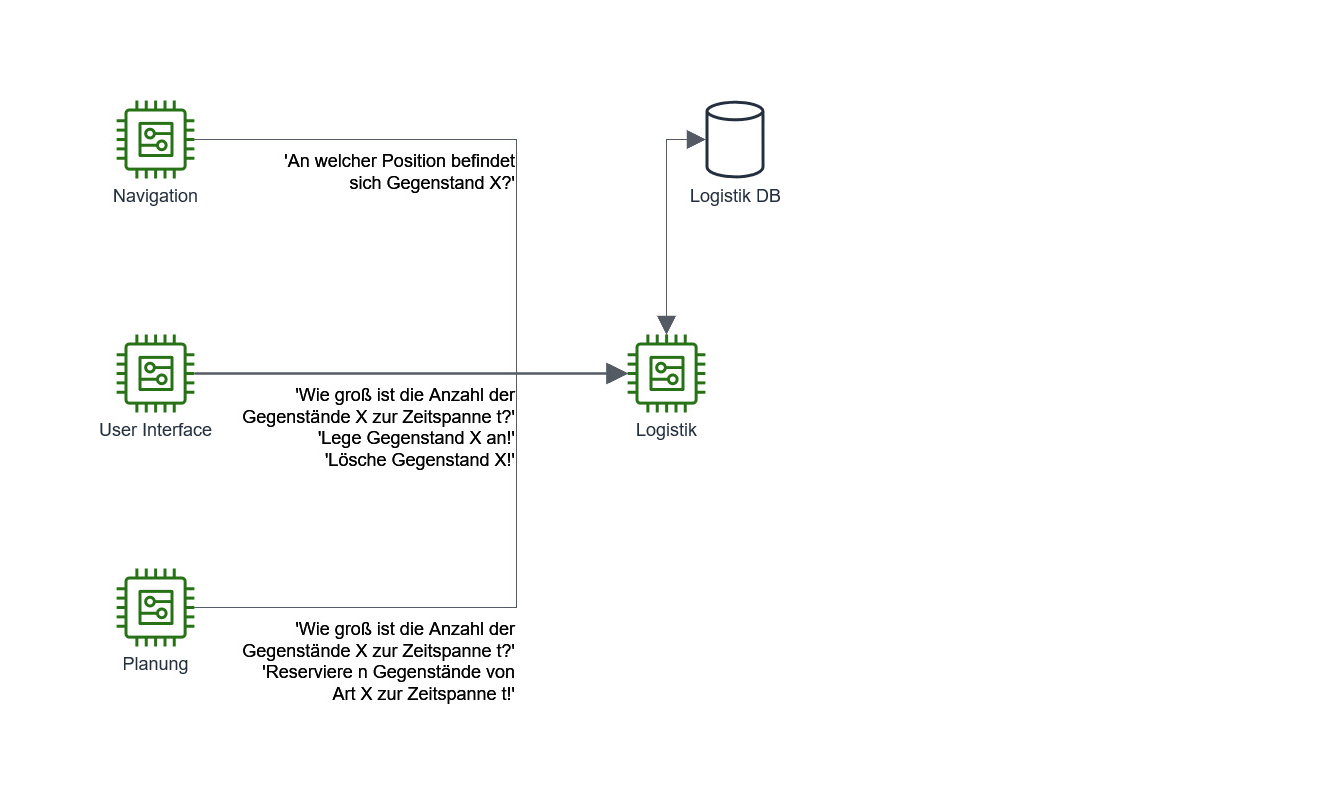
\includegraphics[width=\textwidth]{Bilder/3_Logistik.png}
\caption{Logistik-Knoten}
\end{figure}

Der Logistik-Knoten ist der Einzige, der selbstständig keine Anfragen an andere sendet. Er ist nur für die Kommunikation mit der entsprechenden Datenbank und die Aufbereitung der darin enthaltenen Informationen für andere Knoten verantwortlich. Der Logistik-Knoten kann Anweisungen von allen anderen Knoten erhalten.

Der User Interface-Knoten kann drei verschiedene Anweisungen an den Logistik-Knoten senden. Zum einen kann er erfragen, wie viele Gegenstände einer bestimmten Art zu einer bestimmten Zeitspanne verfügbar sind. Da die Datenbank für jeden Gegenstand Einträge für die blockierten Zeiten besitzt, kann der Knoten eine Datenbank-Anfrage darauf durchführen und die entsprechende Anzahl zurückgeben. Dazu können die Anweisungen kommen, einen neuen Gegenstand anzulegen oder einen bestehenden zu löschen. Beides sind ebenfalls einfache Datenbank-Anfragen, welche der Knoten in einer Rückmeldung mit den Einträgen beantworten kann.

Für die Planung ist es notwendig, dass die Anzahl der verfügbaren Gegenstände zu einer gegebenen Zeitspanne bekannt sind und eingeplante Gegenstände reserviert werden können. Bei einer Reservierung von Gegenständen sucht der Logistik-Knoten die angefragte Anzahl der gegebenen Art aus der Datenbank und fügt der Logistik-Tabelle die entsprechenden Gegenstände hinzu. Dabei müssen die Gegenstände zu dieser Zeitspanne auch verfügbar sein, sodass der Knoten bei der Auswahl die bestehenden Reservierungen mit der angefragten Spanne vergleicht.

Für die Navigation wird davon ausgegangen, dass die Planung korrekt erfolgt ist, bevor die Ausführung der Navigation überlassen wird. Dementsprechend wird von diesem Knoten nur eine Anweisung gesendet, die die derzeitige Position des gesuchten Gegenstands erfragt. Dies ist wieder eine einfache Datenbank-Anfrage, deren Antwort in der Rückmeldung zurückgegeben werden kann.

\begin{table}[h]
\begin{center}
\begin{tabular}{| r l |}
  \hline
  Anweisung  & \dq Wie groß ist die Anzahl der Gegenstände X zur Zeitspanne t?\dq  \\
  \hline
  Rückmeldung & \dq Die Anzahl der Gegenstände X zur Zeitspanne t beträgt n.\dq  \\
  oder     & \textbf{\dq Gegenstand X ist nicht bekannt.\dq } \\
  \hline
  \hline
  Anweisung  & \dq Lege Gegenstand X an!\dq  \\ 
  \hline
  Rückmeldung & \dq Gegenstand X angelegt.\dq  \\  
  oder     & \dq Vorrat X nicht ausreichend.\dq  \\
  oder     & \textbf{\dq Gegenstand X existiert schon.\dq } \\
  \hline
  \hline
  Anweisung  & \dq Lösche Gegenstand X!\dq  \\
  \hline
  Rückmeldung & \dq Gegenstand X gelöscht.\dq  \\
  oder     & \textbf{\dq Gegenstand X ist nicht bekannt.\dq } \\
  \hline
\end{tabular}  
\caption{Kommunikation von User Interface zu Logistik}
\end{center}
\end{table}

\begin{table}[h]
\begin{center}
\begin{tabular}{| r l |}
  \hline
  Anweisung  & \dq Reserviere n Gegenstände von Art X zur Zeitspanne t!\dq  \\
  \hline
  Rückmeldung & \dq Zur Zeitspanne t sind n Gegenstände der Art X reserviert.\dq  \\
  oder     & \textbf{\dq Gegenstand der Art X ist nicht bekannt.\dq } \\
  \hline
\end{tabular}  
\caption{Kommunikation von Planung zu Logistik}
\end{center}
\end{table}

\begin{table}[h]
\begin{center}
\begin{tabular}{| r l |}
  \hline
  Anweisung  & \dq An welcher Position befindet sich Gegenstand X?\dq  \\
  \hline
  Rückmeldung & \dq Gegenstand X befindet sich an Position XY.\dq  \\
  oder     & \textbf{\dq Gegenstand X ist nicht bekannt.\dq } \\
  \hline
\end{tabular}  
\caption{Kommunikation von Navigation zu Logistik}
\end{center}
\end{table}